\documentclass[a4paper]{article}
\usepackage{color}
\usepackage{url}
\usepackage[T2A]{fontenc}
\usepackage[utf8]{inputenc}
\usepackage{graphicx}
\usepackage[english,serbianc]{babel}


\usepackage[unicode]{hyperref}
\hypersetup{colorlinks,citecolor=blue,filecolor=green,linkcolor=blue,urlcolor=blue} 
\renewcommand{\contentsname}{Садржај}

\title{Лични подаци на интернету\\ \small Семинарски рад у оквиру курса\\Техничко и научно писање\\ Математички факултет}

\author{Давид Живковић} 
\begin{document}
\maketitle
\date

\tableofcontents

\newpage

\section{Увод}
\label{sec:увод}
\textbf{Лични подаци} су сви они подаци који се односе на особу, а на основу којих се она може идентификовати (директно или индиректно) и угрозити њена приватност.
\paragraph{}
У времену које карактерише обрада огромне количине најразличитијих података, тзв. „\textbf{ери великих података}”, лични подаци третирају се као „нова нафта”. Своје „бесплатне” услуге компаније наплаћују корисницима тако што им заузврат траже све више личних података. Подаци о корисницима\sloppy, њиховим активностима и понашању на интернету користе се за анализу и креирање личних социјално-психолошких профила, циљано пласирање комерцијалних производа прилагођених индивидуалним карактеристикама и потребама корисника (тзв. „један-на-један маркетинг”), за продају компанијама или сервисима (тзв. „трећим лицима”, eng. \emph {third party}), које те информације углавном користе како би нам доставили што прецизнији саджај како би могли утицати на нас (рекламе, препоручени снимци, итд.). На слици \ref {fig:k} је приказано како изгледа одавање наших података када год ми приступимо интернту са неког уређаја .

\begin{figure}[h!]
\begin{center}
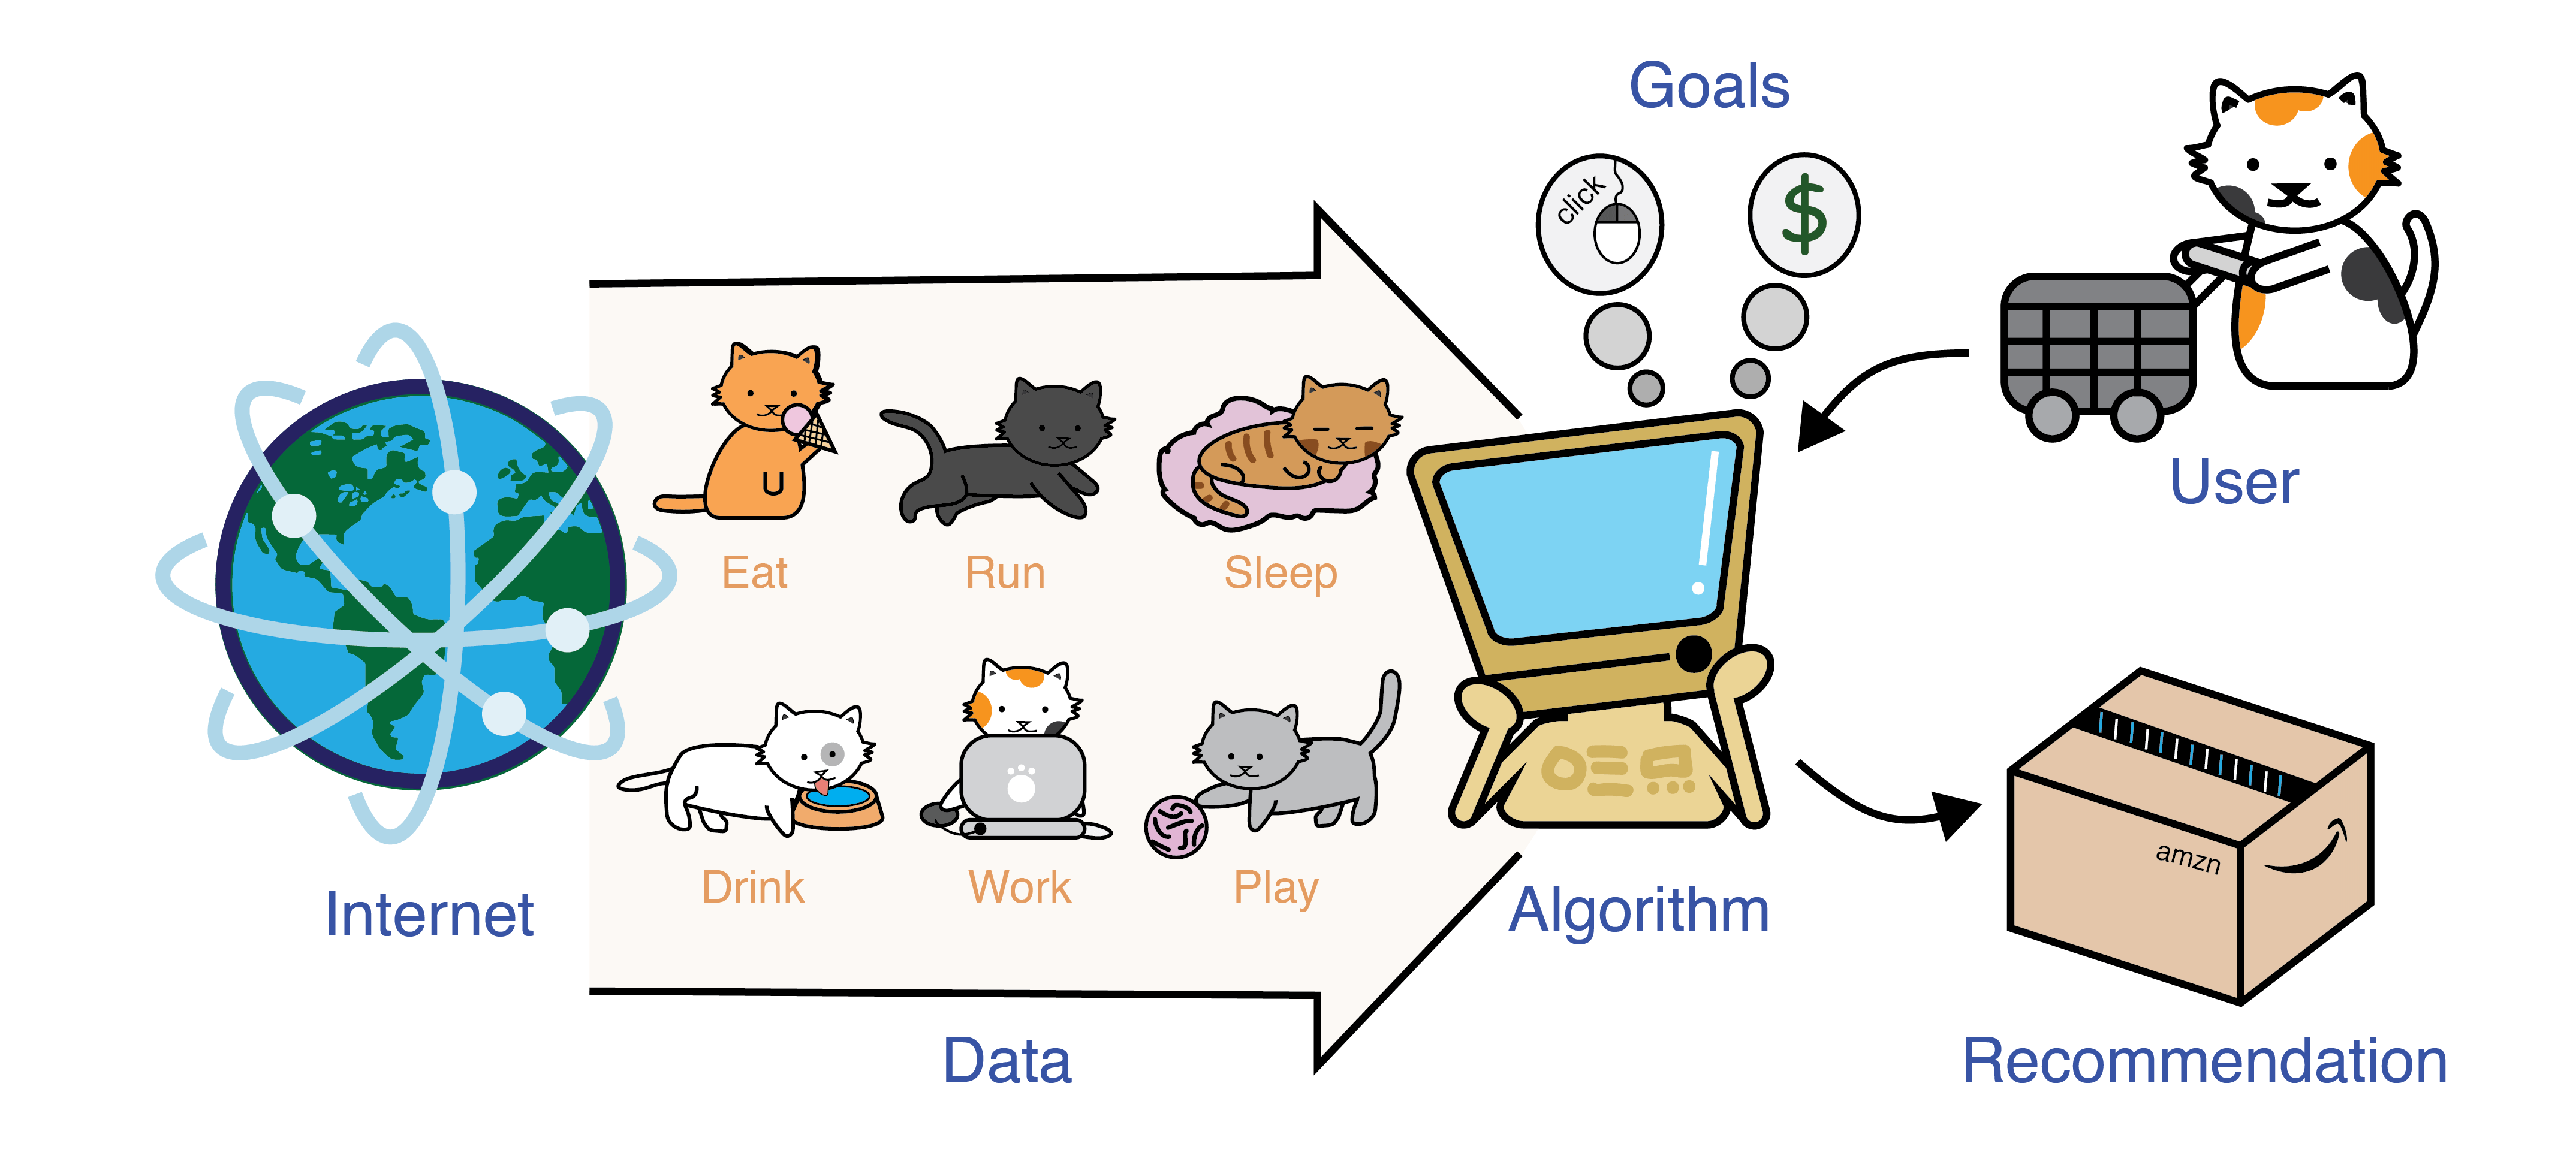
\includegraphics[scale=0.1]{slika2.jpg}
\end{center}
\caption{Кретња наших података}
\label{fig:k}
\end{figure}

\subsection{Kако све остављамо личне податке на интернету}

Сви подаци које ми остављамо се називају \textbf{дигитални отисак}(eng. \emph{Digital print}). Исто као што у форензици на основу наших отисака могу доћи до нас и до података о нама, тако и дигитални отисци служе како би се дала што прецизнија слика о нама и нашим психолошко-социјалним навикама и начинима живота, како би се могло манипулисати нама.

Начини на које ми дајемо своје личне податке(остављамо свој дигитални отисак):

\textbf{Сајтови и онлајн куповина}:
Продавци и сајтови који се баве оцењивањем робе оставе тзв. колачиће (eng. \emph{cookies}) на наш уређај помоћу којих прате наше активности од сајта до сајта, при чему шаљу све чешће рекламе о продуктима које смо недавно гледали.

\textbf{Друштвене мреже}:
Све наше објаве, слике, коментари (чак и они приватни) остављају траг. Због тога треба проверити шта нам је подешено што се тиче приватности на тим платформама. Временом ти сајтови узимају већу слободу при прикупљању наших података, јер се ослањају на то да ће корисници само кликнути „ОК“ када добију обавештење о промени својих правила приватности.

\textbf{Сви уређаји које користимо како бисмо приступили интернету}:
Многи сајтови воде евиденцију о томе са којих све уређаја ми приступамо њиховим сајтовима.


\begin{table}[!h]

\begin{center}

\begin{tabular}{|c|c|} \hline
\textbf{Податак} &\textbf{Проценат успешности}\\ \hline
Пол &93\% \\ \hline
Вера &82\%\\ \hline
Раса & 95\%\\ \hline
Пушач &73\% \\ \hline
Конзумира алкохол &70\% \\ \hline
Користи наркотике & 65\% \\ \hline
Сексуално опредељење &86\% \\ \hline
Политичко опредељење &85\% \\ \hline

\end{tabular}
\label{tab:tabel1}
\caption{Проценат успешности алгоритма}
\end{center}
\end{table}

„\textbf{Лајкови}“, иако наизглед наивни, су веома опасни, наиме Фејсбук је развио алгоритам којим на основу лајкова може закључити о многим информацијама које се тичу корисника, што се може видети у табели \ref {tab:tabel1}.

Бројне личне информације могу бити скривене у фотографијама или видео-садржајима које постављамо на интернет (нпр. име школе, датум рођења, број телефона). Имајте на уму да се много личних података може несмотрено дати и у разговору путем чета или имејла.
\subsubsection{Шерентинг}

Родитељи често несвесно угрожавају право на приватност и безбедност сопствене деце дељењем њихових личних података на интернету (друштвеним мрежама, блоговима). Последњих година све се чешће говори о тзв. \textbf{шерентингу} (eng. \emph{sharenting}), под којим се подразумевају различити начини на које родитељи деле на интернету детаље из приватног живота њихове деце. На тај начин родитељи обликују дигитални идентитет  свог детета много пре него што оно постане самостални корисник интернета. Нажалост, у последње време све се чешће пише о случајевима у којима је објављивање фотографија деце на друштвеним мрежама резултирало негативним искуствима.
    

\section{Врсте личних података}

Под личним подацима подразумевају се:
\paragraph{}
\textbf{Основни подаци}:
име и презиме особе, адреса становања, имејл адреса, фотографија, ИП адреса, локација на којој се особа налази, итд.

\textbf{Подаци који служе за анализу и израду профила корисника}: радне способности, економско стање, лична интересовања, понашање, потрошачке навике, кретање итд.

\textbf{Онлајн понашање особе}: подаци који се прикупљају посредством колачића (поједине компаније су чак почеле и са прикупљањем података о томе како користимо наше уређаје, нпр. којим интензитетом притискамо екран, сваки наш „клик“, па чак и наше покрете мишем, итд.)
\subsection{Врсте личних података на интернету}

Лични подаци на интернету могу се груписати у три категорије:


\begin{itemize}


\item     \textbf{Активни дигитални трагови}: подаци (о себи или другима) које сами корисници остављају приликом коришћења интернета, обично свесно, мада не нужно и намерно  (нпр. приликом куповине неких производа, отварања профила на некој друштвеној мрежи, итд.)
    
\item     \textbf{Пасивни дигитални трагови}: подаци које корисници остављају на интернету приликом његовог коришћења, углавном несвесно (нпр. путем колачића, података о локацији, итд.)
    
\item     \textbf{Подаци добијени анализом првих двеју категорија података}: помоћу алгоритама  (кроз процес профилисања), евентуално у комбинацији са другим изворима података.
Бројне личне информације могу бити скривене у фотографијама или видео-садржајима које постављамо на интернет (нпр. име школе, датум рођења, број телефона).

\end{itemize}
\section{Наша приватност на интернету}

Право на приватност и заштиту личних података јесте једно од основних права прописаних Конвенцијом Уједињених нација о правима детета. Ово право односи се подједнако и на дигитално окружење.
\paragraph{} \textbf{\textit{Приватност није право на тајност, нити на контролу, већ право на одговарајући проток личних података}}\cite{quote}. Шта то конкретно значи? То значи да особа има могућност да, у зависности од ситуације и контекста, лично процени шта ће и са ким делити у \textbf{дигиталном окружењу}. Или, другачије речено, има право да зна како и у које сврхе се користе њени подаци, ко их чува и колико дуго, ко све њима располаже, као и да може да затражи брисање личних података или исправку нетачних података.

    
\subsection{Како да заштитиmo личне податке и приватност на интернету}

Треба имати на уму да је интернет јавни простор и да су лични подаци који се на њему објаве јавно доступни. Приватност на интернету једнако је важна као и ван њега, оно што не бисмо поделили са странцем на улици, не би требало ни на интернету. Неки од начина на које можемо (само до неке мере) заштити наше подактке  су:
	
\begin{itemize}
	
\item     Дељење личних података само са блиским особама, не треба их делити са особама које не познајемо изван интернета.

\item     Упознавање са \textbf{Условима коришћења}(eng. \emph{EULA}\cite{EULA}) и \textbf{Политиком приватности}(eng. \emph{Privacy policy}) пре него што почнемо са коришћењем било које платформе, апликације или сервиса на интернету.
    
\item    Поштовање узрасног ограничења за коришћење интернета, јер самом посетом било које веб-странице се остављају лични подаци на њој.
    

\end{itemize}  

\subsubsection{Како заштити податке детета на интернету}

Велики број веб-сајтова и апликација (нпр. видео-игре, веб-сајтови за друштвено умрежавање или коцкање) траже од корисника да приликом отварања профила наведе свој \textbf{узраст}. На овим сервисима прописана је доња узрасна граница за њихово коришћење.
Да би се избегло добијање родитељске сагласности за млађе од прописаног узраста, већина сервиса поставила је узрасно ограничење за коришћење њихових услуга.

Ово ограничење јасно је наведено у \textbf{Условима коришћења} (које углавном сви занемарују), а од корисника се тражи да се пре почетка коришћења сагласи са овим условима. Како би заштитили корисника, али и себе (избегли кршење закона), веб-сајтови се обавезују да ће обрисати сваки профил који је креирала особа млађа од 13 година. 

Истраживања показују да велики проценат деце (како у свету, тако и у Србији) почиње да користи ове мреже у много ранијем узрасту од прописаног.
Многи родитељи суочавају се са изазовом да ли да дозволе својој деци да отворе профил на некој друштвеној мрежи у узрасту млађем од прописаног. Постати власник личног профила у узрасту млађем од прописаног могуће је само под условом да корисник приликом отварања профила упише погрешан узраст.
Уколико дете приликом отварања профила на неком сервису или друштвеној мрежи наведе да је старије него што јесте, може се десити да:

\begin{itemize}


\item	Буде изложено садржајима који су неприкладни за његов или њен узраст (узнемирујући, насилни или експлицитни).

\item	Изгуби додатне заштите и поставке приватности које се односе на узраст млађи од наведеног.

\item	Лични профил детета, као и сав садржај на њему буду обрисани; осим тога, може му бити онемогућено да отвори лични профил чак и онда када достигне прописани узраст.

\end{itemize}

\section{Закључак}
\paragraph{}

На основу свега наведеног тешко је не забринути се за своју приватност и колико ја она до сад била компромитована. Кад год желимо да приступимо интернету ми одајемо огромну количину својих личних података, а да о томе нисмо ни свесни, мада сада кадa јесмо, да ли то нешто мења? Да ли ћемо ми сад стварно утицати на то колико података одајемо, а колико не, тешко да ћемо ми допринети томе да се о нама зна мање, када се већ до сад све и зна, једино на шта можемо утицати је то да не дозволимо да се нама, као кориснику модерних технологија, не манипулише на основу информација које смо им сами дали.

\begin{thebibliography}{9}


\bibitem{quote} Хелен Нисенбаум, професор инфромационих технологија на Универзитету Корнел https://digitalni-vodic.ucpd.rs/en/personal-data-protection-and-privacy-on-the-internet/
\bibitem{EULA} енг. EULA, End-user license agreement - дигитални уговор између власника софтвера и корисника
\bibitem hhttps://www.pnas.org/content/110/15/5802
\bibitem hhttps://www.ownyourdata.eu/en/blog/
\bibitem hhttps://www.wired.com/story/wired-guide-personal-data-collection/


\end{thebibliography}

\end{document}
